\documentclass[12pt,a4paper,parskip=full]{scrartcl}

\usepackage{bbding}
\usepackage{pifont}
\usepackage{wasysym}
\usepackage[margin=1in]{geometry}
\geometry{letterpaper}
\usepackage{xcolor}
\definecolor{red}{HTML}{cc0000}
\definecolor{gray}{HTML}{666666}
\usepackage{sectsty}
\sectionfont{\color{red}}
\subsectionfont{\color{red}}
\usepackage{graphicx}
\usepackage{hyperref}
\usepackage{amssymb}
\usepackage[style=footnote-dw]{biblatex}
\bibliography{S@SGuideBib}
\setlength\bibitemsep{0.5\baselineskip}

\usepackage{enumitem}
\setitemize{noitemsep}
% \setlist{noitemsep, topsep=-5pt}
% \setlength\itemsep{-0.10em}

\renewcommand{\labelitemi}{$\cdot$}
\renewcommand{\labelitemii}{$\cdot$}
\makeatletter
\let\latexl@section\l@section
\def\l@section#1#2{\begingroup\let\numberline\@gobble\latexl@section{#1}{#2}\endgroup}
\makeatother

\usepackage[T1]{fontenc}
\fontfamily{verdana}

\usepackage{scrlayer-scrpage}{}
\makeatletter
\renewcommand{\@seccntformat}[1]{}
\makeatother

\setlength\parindent{0pt}{}

\title{\Huge{\color{red}\textbf{Le Guide Scrum@Scale
\textsuperscript{\copyright}}}}
\subtitle{\color{gray}Le guide de référence à Scrum@Scale:\\ Une mise à l'échelle qui fonctionne}
% \author{}
\date{}


\begin{document}

%\tableofcontents
%\newpage

\section{Objectif du Guide Scrum@Scale}
Scrum, tel que défini à l’origine dans le Guide Scrum, est un cadre pour développer, livrer
et maintenir des produits complexes par une seule équipe. Depuis sa conception, son
utilisation s’est étendue à des produits, des processus, des services et des systèmes
nécessitant l’effort conjoint de plusieurs équipes. Scrum@Scale a été créé pour
coordonner de façon efficiente ce nouvel écosystème d’équipes de manière à optimiser la
stratégie globale de l’organisation. Cet objectif est atteint en mettant en place une
« bureaucratie minimum viable » au travers d’une architecture sans échelle, qui étend
naturellement la façon dont une équipe fonctionne au sein d’une organisation.

Ce guide contient les définitions des composants du cadre Scrum@Scale, incluant les
rôles à l’échelle d’une organisation, les évènements à l’échelle d’une organisation, et les
artefacts d’entreprise, ainsi que les règles les reliant ensemble.

Le Dr Jeff Sutherland a développé Scrum@Scale en se basant sur les principes
fondamentaux de Scrum, la théorie des systèmes complexes adaptatifs, la théorie des
jeux, et la technologie orientée objet. Ce guide a été développé grâce aux retours
d’expérience de beaucoup de pratiquants Scrum résultant de leurs activités propres.
L’objectif de ce guide est, pour le lecteur, d’être capable d’implémenter Scrum@Scale de
façon autonome.

\subsection{Pourquoi Scrum@Scale ?}
Scrum a été conçu pour qu’une équipe seule soit capable de travailler à sa capacité
optimale tout en maintenant un rythme soutenable. Il s’avère qu’à mesure que le nombre
d’équipes Scrum grandit dans une organisation, le résultat optimal (le produit opérationnel)
et la vélocité de ces équipes commencent à baisser (du fait des problèmes liés aux
dépendances inter-équipe et à la duplication du travail). Il est devenu évident qu’un cadre
pour coordonner efficacement ces équipes soit nécessaire pour supporter cette
extensibilité linéaire. Scrum@Scale est conçu pour atteindre cet objectif grâce à son
architecture libre de toute échelle.

En utilisant une architecture libre d’échelle, une organisation n’est pas contrainte à une
croissance particulière qui serait déterminée par un ensemble de règles arbitraires. Au lieu
de cela, elle peut croitre de façon organique en se basant uniquement sur ses propres
besoins et à un rythme de changement soutenable facilitant ainsi son acceptation par les
différents groupes d’individus qui constituent l’organisation.

Scrum@Scale est conçu pour s’étendre sur l’ensemble de l’organisation : tous
départements, produits et services confondus. Il peut s’appliquer à de multiples domaines
dans tous types d’organisations industrielles, gouvernementales ou académiques.

\subsection{Définition de Scrum@Scale}
Scrum (n) : Cadre dans lequel les gens peuvent gérer des problèmes complexes et
adaptatifs tout en produisant efficacement et avec créativité des produits ayant la plus
forte valeur possible.

Le Guide Scrum présente les caractéristiques minimales permettant l’inspection et
l’adaptation au travers d’une transparence drastique pour piloter l’innovation, la
performance, et le bien-être de l’équipe.

Scrum@Scale (n) : Cadre dans lequel un réseau d’équipes Scrum opèrent en cohérence
avec le Guide Scrum pour gérer des problèmes complexes et adaptatifs tout en produisant
avec créativité des produits ayant la plus forte valeur possible.

\textbf{REMARQUE:} Ces « produits » peuvent être du matériel, du logiciel, des systèmes
complexes, des processus, des services, etc… en fonction du domaine des équipes
Scrum.

Scrum@Scale est:
\begin{itemize}
\item Léger – la bureaucratie minimum viable
\item Simple à comprendre – Consistant uniquement en équipes Scrum
\item Difficile à maîtriser – requière l’implémentation d’un nouveau modèle opérationnel
\end{itemize}


Scrum@Scale est un cadre pour faire du Scrum à grande échelle. Il simplifie radicalement
le passage à grande échelle par l’utilisation de Scrum pour passer Scrum à grande
échelle. Ce cadre se compose uniquement d’équipes Scrum coordonnées via des Scrum
de Scrums et des MetaScrums.

La nature de Scrum@Scale basée sur des composants permet à une organisation de
personnaliser sa stratégie de transformation et sa mise en oeuvre. Il leur fournit la
possibilité de cibler leurs efforts de transformation sur le(s) domaine(s) le(s) plus
important(s) ou ayant le plus besoin de changements, puis progresser sur d’autres
ensuite.

Dans Scrum, une attention est portée à séparer la responsabilité du `` quoi '' et du
`` comment ''. La même attention est portée dans Scrum@Scale afin que compétence et
responsabilité soient clairement comprises pour éliminer tout conflit organisationnel inutile
rendant les équipes moins enclines à atteindre leur productivité optimale.

En liaison avec la séparation de ces deux champs de compétences, Scrum@Scale
présente deux cycles : le cycle Scrum Master (le `` comment '') et le cycle Product Owner
(le `` quoi ''), les deux se recoupant en deux points. Conjointement, ces deux cycles
donnent un cadre puissant pour coordonner les efforts de plusieurs équipes sur une seule
et même voie.

\subsection{Les Composants du cadre de Scrum@Scale\textregistered ~}

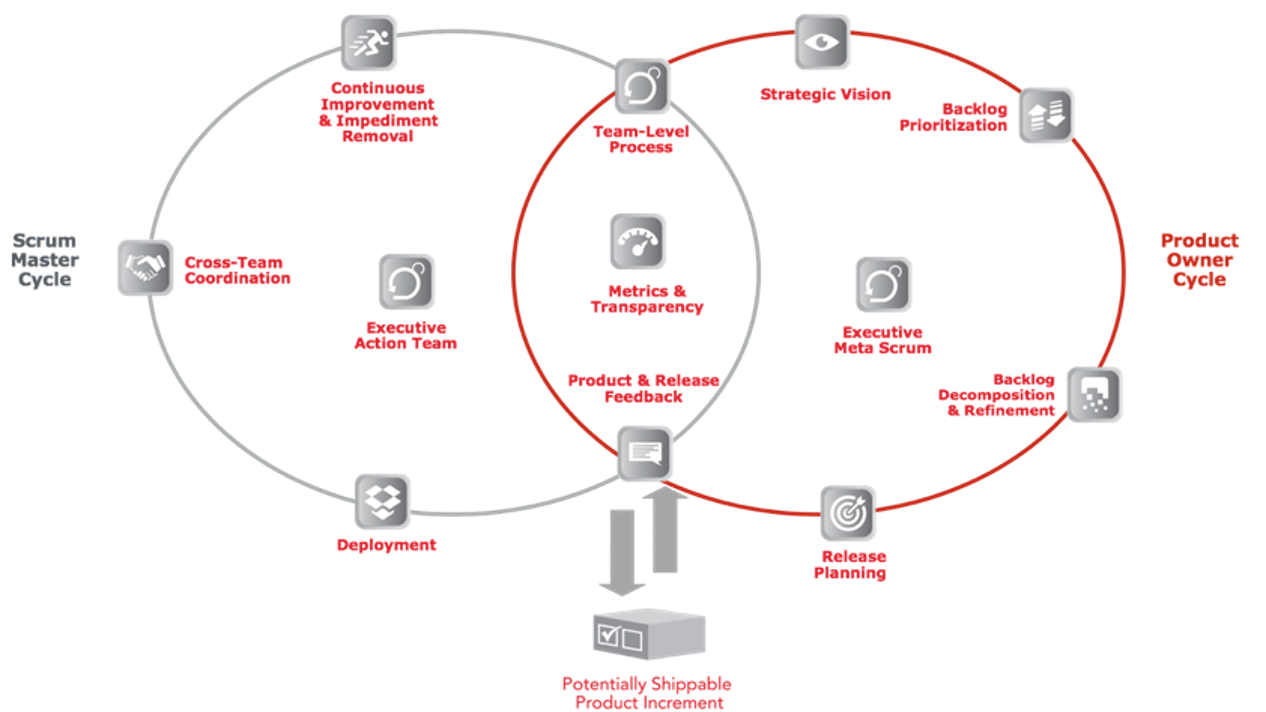
\includegraphics[width=1.0\linewidth]{Cycle-SMPO.png}

\subsection{Culture Pilotée par les Valeurs}
En plus de séparer la responsabilité du `` quoi '' et du `` comment '', Scrum@Scale vise
également à construire des organisations saines en créant une culture axée sur des
valeurs dans un cadre empirique. Les valeurs de Scrum sont : Focalisation, Ouverture,
Respect, Courage et Engagement. Ces valeurs orientent une prise de décision empirique,
cette dernière repose sur trois piliers que sont la transparence, l'inspection et l'adaptation.

L'Ouverture favorise la transparence dans tous les travaux et processus, sans laquelle il
n'y aurait aucune possibilité de pouvoir les inspecter honnêtement et de tenter de les
adapter pour le mieux. Le Courage se réfère aux sauts audacieux requis pour fournir de la
valeur plus rapidement de manière innovante.

La Focalisation et l’Engagement se réfèrent à la manière dont nous gérons nos obligations
professionnelles, en accordant la plus haute priorité à la livraison de la valeur client. Enfin,
tout cela doit se faire dans un environnement basé sur le respect des personnes qui font le
travail, sans qui rien ne peut être créé.

Scrum@Scale aide les organisations à se développer en soutenant un modèle de
leadership axé à la fois sur la collaboration et l'intention\footnote{Marquet, L
David, Turn the Ship Around!: How to Create Leadership at Every Level,
Greenleaf Book Group, 2012}, en favorisant un environnement
positif pour travailler à un rythme soutenable et en s'engageant à offrir la valeur client
comme première préoccupation au centre de nos efforts.

\subsection{Premiers pas avec Scrum@Scale}
Lors de la mise en oeuvre de grands réseaux d'équipes, il est essentiel de développer un
\textbf{modèle de référence} évolutif pour un petit nombre d'équipes. Toute lacune dans une
mise en oeuvre Scrum sera amplifiée lorsque plusieurs équipes seront déployées.

Par conséquent, le premier défi consiste à créer un petit groupe d'équipes qui implémente
bien Scrum. Cet ensemble d'équipes traite les problèmes organisationnels qui bloquent
l'agilité et crée un modèle de référence pour Scrum connu pour fonctionner dans
l'organisation et pouvant être utilisé comme modèle pour la mise à l'échelle de Scrum à
travers l'organisation.

À mesure que le modèle de référence des équipes s'accélère, les obstacles et les goulets
d'étranglement qui retardent la livraison, génèrent du gaspillage ou entravent l'agilité
commerciale deviennent évidents. Le moyen le plus efficace d'éliminer ces problèmes
consiste à répartir Scrum à travers l'organisation afin que la totalité de la chaîne de valeur
soit optimisée.

Scrum@Scale permet d’obtenir une augmentation linéaire de la productivité en saturant
l'organisation avec Scrum et en distribuant organiquement la vélocité et la qualité, tout
cela en cohérence avec la stratégie, les produits et les services spécifiques de
l'organisation.

\section{Le cycle Scrum Master}
\subsection{Le processus au niveau de l’équipe}
Le \textbf{processus au niveau de l’équipe} est clairement expliqué dans le Guide Scrum. Ce
processus est composé de 3 artefacts, cinq évènements, et trois rôles. Les objectifs du
processus au niveau de l’équipe sont de :
\begin{itemize}
\item Maximiser le flux de travail terminé et ayant un niveau de qualité vérifié.
\item Augmenter petit à petit la vélocité Sprint après Sprint.
\item Travailler de manière durable et enrichissante pour l’équipe.
\end{itemize}

\subsection{Coordonner le `` Comment '' - Le Scrum de Scrums}
Lorsqu’un ensemble d’équipes a besoin de se coordonner, elles forment un \textbf{« Scrum de
Scrums » (SdS)}. Un SdS est une « équipe d’équipes »\footnote{McChrystal, General Stanley and Collins, Tantum and
Silverman, David and Fussell, Chris, Team of teams: New rules of engagement
for a complex world, Penguin, 2015} qui se réunit lors d’un événement
dénommé Mêlée Quotidienne Élargie (MQE) avec un représentant de chaque équipe
(généralement le Scrum Master de chaque équipe, même si n’importe quel membre de
l’équipe peut y participer). La MQE existe pour coordonner les équipes et supprimer les obstacles à la livraison 
de valeur.

L’évènement de la MQE est le pendant de la Mêlée Quotidienne dans le sens où elle
optimise la collaboration et la performance d’un réseau d’équipes. En outre, la MQE:

\begin{itemize}
\item A une durée limitée à 15 minutes ou moins.
\item Doit réunir un représentant de chaque équipe.
\item Est un forum où les représentants des équipes doivent répondre à 3 questions
simples :
\begin{itemize}
\item Quels sont les obstacles auxquels mon équipe est confrontée et qui sont en
mesure de l’empêcher d’atteindre ses Objectifs de Sprint (ou qui auront des
impacts sur la version à venir) ?
\item Est-ce que mon équipe est en train de faire quelque chose qui pourrait
empêcher une autre équipe d’atteindre ses Objectifs de Sprint (ou qui auront
des impacts sur la version à venir) ?
\item Avons-nous découvert une nouvelle dépendance inter-équipes ou découvert
un moyen de résoudre une dépendance répertoriée ?
\end{itemize}
\end{itemize}
Cette équipe de Scrum Masters est une Équipe Scrum à part entière, responsable d’un
ensemble complètement intégré d’incréments potentiellement livrables d’un produit à la fin
de chaque Sprint issus de toutes les équipes participantes. L’équipe du SdS doit être
réactive en temps réel quant aux obstacles remontés par les équipes participantes.

Un SdS fonctionne comme une équipe de livraison et doit être en capacité de livrer
directement de la valeur aux clients. Pour le faire de manière efficace, elle doit travailler
conformément au Guide Scrum ; c’est-à-dire avoir ses propres rôles, artefacts et
évènements. Cela comprend l’évènement d’Affinage de Backlog dans lequel elle décide
quels sont les obstacles « prêts » à être supprimés, quelle est la meilleure manière de les
supprimer et de quelle manière l’équipe saura que c’est bien « fini ». Une attention
particulière devra être portée à la Rétrospective du SdS dans laquelle les représentants
des différentes équipes partagent ce qu’ils ont appris ou les améliorations de processus
que leur équipe respective a été en mesure de faire dans l’objectif de standardiser les
pratiques entre les équipes du SdS.

Le SdS doit avoir toutes les compétences nécessaires pour livrer un produit complètement
intégré potentiellement livrable à la fin de chaque Sprint. Le Product Owner doit également
être présent ou représenté afin de résoudre les problèmes de priorisation. Des architectes,
des testeurs et tout autre personne ayant des compétences opérationnelles utiles peuvent
s’avérer nécessaires.\footnote{Lorsqu’elles commencent Scrum@Scale les équipes n’ont peut-être pas
l’infrastructure pour pouvoir faire du déploiement continu. Cela devrait forcer le SdS à
mettre en place une « équipe d’intégration » ou une « équipe de livraison » qui fera le
travail supplémentaire nécessaire pour pallier aux manques d’ingénierie. Par exemple,
Amazon a près de 1 000 équipes Scrum qui livrent de nouvelles fonctionnalités en
production toutes les secondes sans équipe d’intégration. Le retour sur investissement
de cette automatisation pour permettre le déploiement en continu est de l’ordre de 72
000 % (Rico, 2017). Ce retour sur investissement astronomique forcera finalement
toutes les autres entreprises à investir pour automatiser pour rester compétitive.}.

\subsection{Le Scrum de Scrums Master (SdSM)}
Le Scrum de Scrums Master est responsable pour le déploiement de l’effort commun et
doit :
\begin{itemize}
\item Rendre visible le backlog des obstacles aux yeux de l’organisation.
\item Supprimer les obstacles que les équipes ne sont pas en mesure de résoudre
elles-mêmes.
\item Prioriser les obstacles, avec une attention particulière aux dépendances interéquipes
et la distribution du backlog.
\item Améliorer l’efficacité du Scrum de Scrums.
\item Travailler étroitement avec les Product Owners pour déployer un Incrément de
Produit potentiellement livrable au moins à chaque Sprint.
\item Coordonner le déploiement des équipes avec les Plans de Versions du Product
Owner.
\end{itemize}

\subsection{Le SdS à l’échelle}
Selon la taille de l’organisation ou de l’implémentation, il peut être nécessaire d’avoir plus
d’un SdS pour livrer un produit très complexe. Dans ce cas, un \textbf{Scrum de Scrum de
Scrums (SdSdS)} peut être mis en place à partir de l’ensemble des Scrums de Scrums. Le
SdSdS est un schéma d’organisation organique d’équipes qui peut être élargit
indéfiniment. Chaque SdSdS devrait avoir un SdSdSM et des versions élargies de chaque
artefact et événement.

Élargir le SdS permet de réduire les canaux de communication au sein de l’organisation
afin que la complexité reste confinée. Le SdSdS s’interface avec un SdS de la même
manière qu’un SdS s’interface avec une seule équipe Scrum permettant ainsi un
élargissement linéaire.

\pagebreak
Exemple de diagrammes :

\includegraphics[width=1.0\linewidth]{Sds-R2.png}

\textbf{\textsc{REMARQUE:}} Alors que le Guide Scrum définit la taille optimale de l’équipe entre 3 et 9
personnes, les résultats d’une recherche à Harvard montre que la taille optimale d’une
équipe est 4,6 personnes.\footnote{Hackman, J Richard, Leading teams: Setting the stage for
great performances, Harvard Business Press, 2002} Il a été prouvé lors de différentes expériences que la taille des
équipes Scrum s’étant montrées parmi les plus productives était comprise entre 4 et 5
personnes. Dans le cadre d’un élargissement linéaire, il est essentiel que le nombre de
personnes présentes dans les équipes d’un SdS suivent ce même schéma. Par
conséquent, dans les diagrammes précédents et dans ceux qui vont suivre, la forme du
pentagone a été choisie pour représenter une équipe de 5 personnes. Ces diagrammes
sont seulement donnés uniquement à titre d’exemple, les diagrammes de votre
organisation peuvent bien sûr être différents.

\subsection{L’Équipe Opérationnelle Exécutive (EOE)}
Le Scrum de Scrum qui intervient au niveau de l’ensemble de l’organisation agile porte le
nom de \textbf{Équipe Opérationnelle Exécutive (EOE)}. L’EOE est là pour mettre un point final
aux obstacles qui ne peuvent pas être supprimés par le SdS qui l’a détecté. Par
conséquent, elle doit être composée d’individus ayant le pouvoir politique et financier pour
les supprimer. La fonction de l’EOE est de coordonner les différents SdS (ou les SdSdS).
Comme dans n’importe quelle autre équipe Scrum, elle a besoin d’un PO et d’un SM. Il est
préférable que l’EOE se réunisse quotidiennement comme toute autre équipe Scrum. Elle
doit se réunir au minimum une fois par Sprint et avoir un backlog qui soit transparent.
Exemple de diagramme d’une EOE coordonnant 5 groupes de 125 équipes au total :

\pagebreak
Exemple de diagramme montrant un EOE coordonnant 5 groupes de 25 équipes:

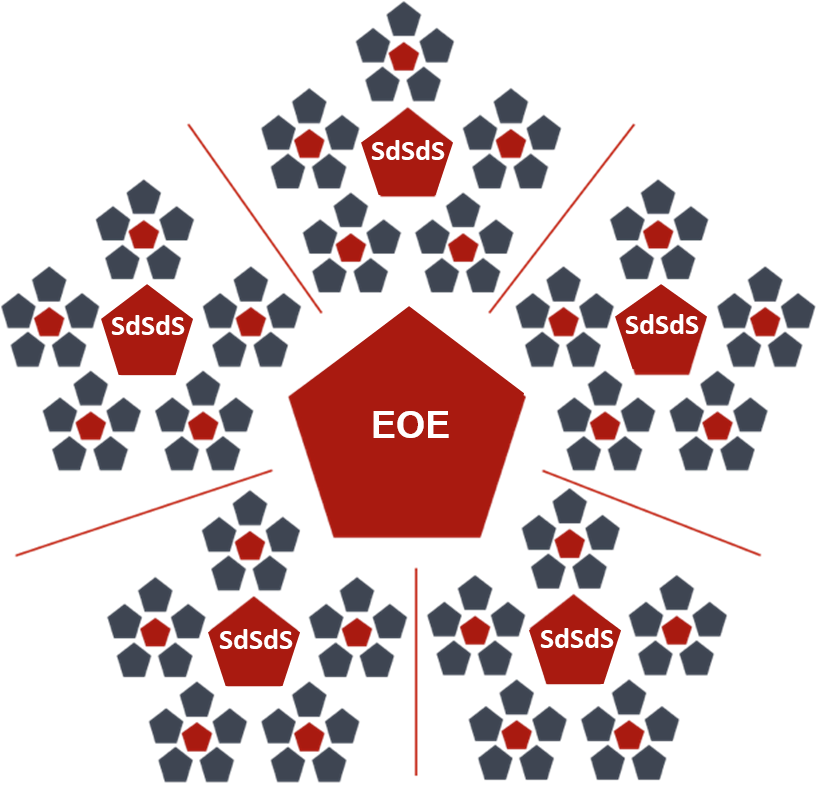
\includegraphics[width=1.0\linewidth]{SdS-EOE.png}

\subsection{Backlog \& responsabilités de l’EOE}
Scrum est un système d’exploitation agile différent de la gestion de projet traditionnelle.
L’ensemble des SMs de l’organisation rend compte à l’EOE qui est responsable de la mise
en place du système d’exploitation agile en établissant, maintenant et améliorant son
implémentation dans l’organisation.

Le rôle de l’EOE est de créer le Backlog de Transformation Organisationnelle (une liste
priorisée d’initiatives agiles qui doivent être réalisées) et d’examiner ce qui est mener à
bien. Par exemple, s’il y a un cycle de vie traditionnel de développement des produits dans
l’ancienne organisation, un nouveau cycle de vie de développement des produits doit être
créé, implémenté et soutenu. De manière générale, cela donnera de meilleurs résultats au
niveau des problèmes de qualité et de conformités que l’ancienne méthode mais sera
implémenté de manière différente avec des règles différentes et des orientations
générales différentes. Il y a beaucoup d’autres aspects organisationnels au niveau du
développement et de la gouvernance qui pourraient avoir besoin de nouveaux réglages.

L’EOE est responsable de la qualité de Scrum dans l’organisation. Ses responsabilités
comportent de manière non exhaustive :
\begin{itemize}
\item Créer un système d’exploitation agile qui soit le Modèle de Référence pour
s’étendre sur l’ensemble de l’organisation, y compris les règles, procédures et
lignes directrices d’entreprises à un niveau opérationnel permettant d’établir
l’agilité.
\item Mesurer et améliorer la qualité de Scrum au sein de l’organisation.
\item Construire la capacité au sein de l’organisation de l’agilité métier.
\item Créer un centre pour l’apprentissage continu des professionnels de Scrum.
\item Soutenir l’exploration de nouvelles manières de travailler.
\end{itemize}
Finalement, l’EOE doit mettre en place et soutenir une organisation de Product Owners à
travers l’association de PO qui puissent être l’équivalent du Scrum de Scrum et étendre
leurs fonctions de PO. Ces équipes de PO et de parties prenantes clés portent le nom de
\textbf{MetaScrums}.

\subsection{Résultats produits/Effets produits de l’organisation Scrum
Master}
L’organisation Scrum Master (SdS, SdSdS, et EOE) travaille comme un tout qui permet de
compléter le Cycle du Scrum Master : \textbf{Amélioration Continue et Suppression des
Obstacles, Coordination Inter-Équipes et Déploiement}.

Les objectifs de l’Amélioration Continue et de la Suppression des Obstacles sont :
\begin{itemize}
\item Identifier les obstacles et les réinterpréter comme des opportunités.
\item Maintenir un environnement sûr et structuré pour prioriser et supprimer les
obstacles, puis vérifier les améliorations qui en résultent.
\item Assurer une visibilité au niveau de l’organisation pour effectuer les
changements.
\end{itemize}
Les objectifs de la Coordination Inter-Équipes sont :
\begin{itemize}
\item Coordonner les processus similaires à travers différentes équipes qui sont en
relation les unes avec les autres.
\item Gérer les dépendances inter-équipes pour s’assurer qu’elles ne deviennent pas
des obstacles.
\item Maintenir l’alignement des normes et des lignes directrices des équipes afin
d’obtenir des résultats cohérents.
\end{itemize}

Étant donné que le but du SdS est de fonctionner comme une équipe de livraison, le
déploiement du produit est donc dans son périmètre, tandis que le contenu des
différentes livraisons est dans celui des Product Owners. Par conséquent, les objectifs
du Déploiement sont :
\begin{itemize}
\item Livrer un flux constant de produits finis ayant de la valeur pour les clients.
\item Intégrer le travail de différentes équipes de manière homogène dans un produit
unique.
\item Assurer une expérience client de très grande qualité.
\end{itemize}

\section{Le cycle du Product Owner}
\subsection{Coordonner le « Quoi » - Le MetaScrum}
Un textbf{MetaScrum} est le nom donné à un groupe de Product Owners ayant besoin de
coordonner un backlog unique qui viendra alimenter un Scrum de Scrums. À chaque SdS
est associé un MetaScrum. Un MetaScrum permet d’aligner les priorités des différentes
équipes sur une seule vision afin qu’elles puissent coordonner leurs backlogs respectifs et
créer cet alignement avec les parties prenantes. Les MetaScrums maintiennent une
version élargie de l’Affinage du Backlog.
\begin{itemize}
\item Chaque PO d’équipe (ou son proxy) doit y assister
\item Cet événement constitue le forum de la Direction, des parties prenantes et
autres Clients pour exprimer leurs préférences
\end{itemize}
Cet événement se déroule aussi souvent qu’il se doit, au moins une fois par Sprint, dans
l’objectif d’avoir un backlog Prêt. Les fonctions du MetaScrum sont de :
\begin{itemize}
\item Créer une vision globale du produit & la rendre visible au niveau de
l’organisation.
\item Bâtir l’alignement des parties prenantes clés pour sécuriser l’implémentation du
backlog.
\item Produire un backlog unique priorisé afin d’éviter une duplication des travaux de
développement.
\item Créer une « Définition de Fini » uniforme qui s’appliquera à toutes les équipes
du SdS.
\item Éliminer les dépendances soulevées par le SdS.
\item Produire un Plan de Version coordonné.
\item Identifier et surveiller les métriques donnant un aperçu du produit.
\end{itemize}
Les MetaScrums, comme les SdS, fonctionnent comme des équipes Scrum à part entière.
En tant que tel, ils ont besoin de quelqu’un qui puisse agir en tant que SM et veille à
maintenir l’équipe sur la bonne voie dans les discussions et de quelqu’un qui soit
responsable de coordonner l’alimentation du Product Backlog unique pour l’ensemble des
équipes concernées par le MetaScrum. Cette personne est désignée sous le nom de \textbf{Chef
Product Owner}.

\subsection{Le Chef Product Owner (CPO)}
À travers les MetaScrums, les Chefs Product Owners coordonnent les priorités des
Product Owners qui travaillent auprès des différentes équipes. Ils alignent les priorités du
backlog avec les besoins des Parties Prenantes et des Clients. De la même manière que
le SdSM, les Chefs Product Owners peuvent être une équipe à part entière de PO qui
choisit de jouer également ce rôle, ou cela peut être une personne spécialement dédiée à
ce rôle. Ses principales responsabilités sont les mêmes que pour un PO ordinaire mais sur
une échelle plus large :
\begin{itemize}
\item Mettre en place une vision stratégique pour l’ensemble du produit.
\item Créer un seul backlog priorisé de la valeur à livrer par toutes les équipes.
\begin{itemize}
\item Ces items seront des stories plus grosses que les stories ordinaires.
\end{itemize}
\item Travailler étroitement avec les SdSM associés afin que le Plan de Version que
l’équipe MetaScrum a créé puisse être déployé de manière efficiente.
\item Suivre les retours des utilisateurs du produit et ajuster le backlog en
conséquence.
\end{itemize}

\subsection{Élargir le MetaScrum}
De la même manière qu’un SdS peut s’agrandir en SdSdS, les MetaScrums peuvent
s’agrandir selon un mécanisme similaire. Il n’existe pas de terme spécifique associé à ces
unités élargies, ni non plus pour les Chefs Product Owners. Nous encourageons chaque
organisation à développer ses propres termes. Dans les diagrammes suivants, nous
avons choisi d’ajouter le terme « Chef » aux titres des PO pour les faire ressortir.

%\pagebreak
Quelques diagrammes en exemple :

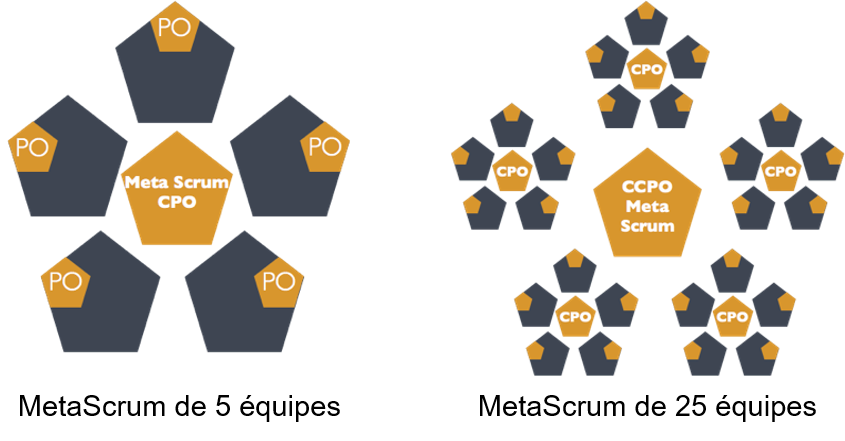
\includegraphics[width=1.0\linewidth]{MetaScrum-R2.png}

\textbf{REMARQUE:} Comme mentionné précédemment, ces pentagones représentent la taille
idéale des équipes Scrum et la taille idéale des MetaScrums. Ces diagrammes sont
donnés uniquement à titre indicatif, vos diagrammes organisationnels peuvent s’avérer
très différents.

\subsection{Le MetaScrum Exécutif (MSE)}
Les MetaScrums permettent une conception en réseau de Product Owners qui est
évolutif à l'infini en même temps que les SoS associés. Le MetaScrum pour l'ensemble
de l'organisation agile est le \textbf{MetaScrum Exécutif}. Le MSE possède la vision
organisationnelle et définit les priorités stratégiques pour l'ensemble de l'entreprise, en
alignant toutes les équipes autour d'objectifs communs.

Exemples de diagrammes montrant un MSE coordonnant 5 groupes de 25 équipes :

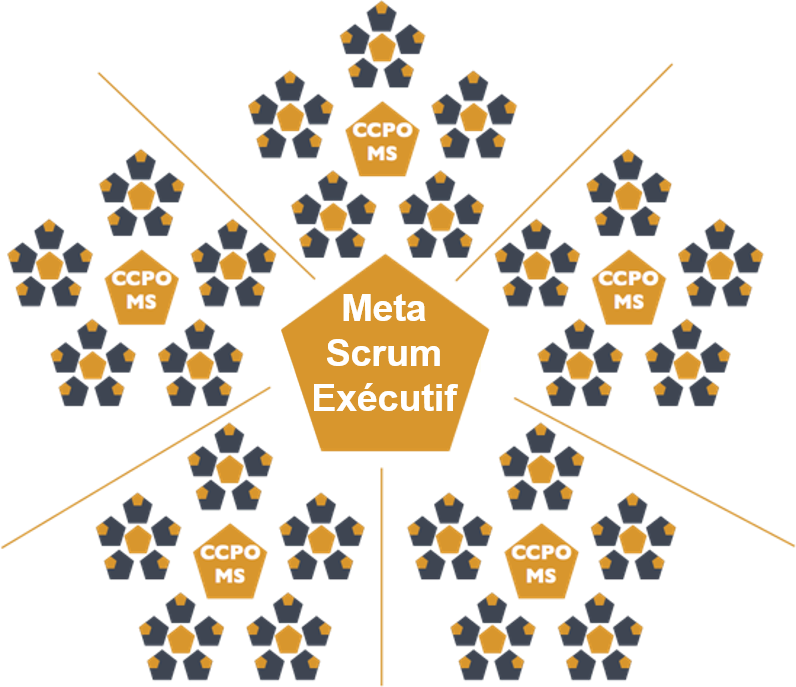
\includegraphics[width=1.0\linewidth]{MetaScrumExecutif.png}

\subsection{Résultats produits/Effets produits de l’Organisation Product
Owner}
L'organisation PO (les différents MetaScrums, le CPO et le MetaScrum Exécutif)
travaille dans son ensemble pour satisfaire les composants du cycle Product Owner:
\textbf{Vision Stratégique, Priorisation des Backlogs, Décomposition et Affinage des
Backlogs et Planification des Versions.}.

Les objectifs d’une Vision Stratégique sont :
\begin{itemize}
\item Aligner clairement l’organisation dans son ensemble sur une vision partagée.
\item Expliquer de manière convaincante pourquoi l'organisation existe.
\item Décrire ce que l'organisation fera pour tirer parti des atouts clés à l'appui de sa
mission.
\item Mettre à jour continuellement pour répondre à l'évolution rapide des conditions
du marché.
\end{itemize}
Les objectifs de la Priorisation du Backlog sont :
\begin{itemize}
\item Identifier une commande claire pour les produits, les fonctionnalités et les
services à livrer.
\item Refléter la création de valeur, l'atténuation des risques et les dépendances
internes dans la gestion du backlog.
\item Prioriser les initiatives de haut niveau dans l'ensemble de l'organisation agile
avant la Décomposition et l’Affinage du Backlog.
\end{itemize}
L’objectif de la Décomposition et de l’Affinage du Backlog sont :
\begin{itemize}
\item Diviser les projets et les produits complexes en éléments fonctionnels
indépendants pouvant être complétés par une équipe dans un Sprint.
\item Capturer et distiller les exigences émergentes et les retours des clients.
\item S'assurer que tous les items du backlog sont vraiment « prêts » afin qu'ils
puissent être pris en charge par les équipes individuelles.
\end{itemize}
Les objectifs de la Planification des Versions sont :
\begin{itemize}
\item Prévoir la livraison des fonctionnalités et capacités clés.
\item Communiquer les prévisions de livraison aux parties prenantes.
\item Mettre à jour les priorités, au besoin.
\end{itemize}

\section{Connecter les cycles PO/SM}

\subsection{Comprendre les Retours d’Information}
Le composant \textbf{Retour d’Information} est le second point où les cycles PO et SM se
recoupent. Les retours d’information sur le Produit entrainent l’amélioration continue en ajustant le
Backlog de Produit tandis que les retours d’information de Version entraînent
l’amélioration continue en ajustant les mécanismes de Déploiement. Les objectifs de
l’obtention et l’analyse des Retours d’Information sont :
\begin{itemize}
\item Valider les hypothèses.
\item Comprendre comment les clients utilisent le produit et interagissent avec lui.
\item Capturer de nouvelles idées de caractéristiques et fonctionnalités.
\item Définir les améliorations des fonctionnalités existantes.
\item Mettre à jour la progression du produit/projet pour affiner le planning de versions et
l’alignement des parties-prenantes.
\item Identifier les améliorations des méthodes et mécanismes de déploiement.
\end{itemize}

\subsection{Métriques \& Transparence}
La transparence radicale est essentielle pour que Scrum fonctionne de manière
optimale, mais cela n'est possible que dans une organisation qui a adopté les valeurs
Scrum. Elle donne à l'organisation la capacité d'évaluer honnêtement ses progrès et
d'inspecter et d'adapter ses produits et processus. C'est le fondement de la nature
empirique de Scrum tel que décrit dans le Guide Scrum.

Les deux cycles SM et PO exigent des métriques qui seront décidées par chacune des
organisations SM et PO. Les métriques peuvent être propres à des organisations
spécifiques ainsi qu'à des fonctions spécifiques au sein de ces organisations.
Scrum@Scale ne nécessite aucun ensemble spécifique de métriques, mais suggère que,
au strict minimum, l'organisation doit mesurer :
\begin{itemize}
\item La productivité – i.e. les changements en termes de volume de Produit
Opérationnel livré par Sprint
\item La Valeur Produite – i.e. la valeur métier par unité d’effort d’équipe
\item La Qualité – i.e. taux de défauts ou temps d’arrêt de service
\item La Soutenabilité – i.e. le bienêtre de l’équipe
\end{itemize}
Les objectifs de ces métriques et de la transparence sont :
\begin{itemize}
  \item Fournir à tous les décideurs, y compris les membres de l'équipe, le contexte
approprié pour prendre de bonnes décisions.
\item Raccourcir autant que possible les cycles de retour d’information afin d'éviter
une correction excessive.
\item Necessiter un effort supplémentaire minimal de la part des équipes, des parties
prenantes ou du leadership.
 \end{itemize}

\subsection{Quelques remarques sur la conception d’organisation}
La nature libre d’échelle de Scrum@Scale permet une conception de l'organisation
basée sur des composants, tout comme le cadre lui-même. Cela permet de
rééquilibrer ou de restructurer des équipes en réponse au marché. Au fur et à mesure
que l'organisation se développe, il peut être important de saisir les avantages des
équipes distribuées. Certaines organisations arrivent à attirer des talents qui seraient
autrement indisponibles et sont en mesure de se développer et de se contracter selon
les besoins grâce à un développement externalisé. Scrum@Scale montre comment
faire cela tout en évitant d’allonger les délais, de détériorer les communications et
réduire la qualité, en permettant une évolutivité linéaire à la fois en taille et en
distribution globale.\footnote{Sutherland, Jeff and Schoonheim,
Guido and Rustenburg, Eelco and Rijk, Maurits, "Fully distributed scrum:
The secret sauce for hyperproductive offshored development teams",
AGILE'08. Conference, IEEE: 339-344, 2008}

Quelques exemples de diagrammes :
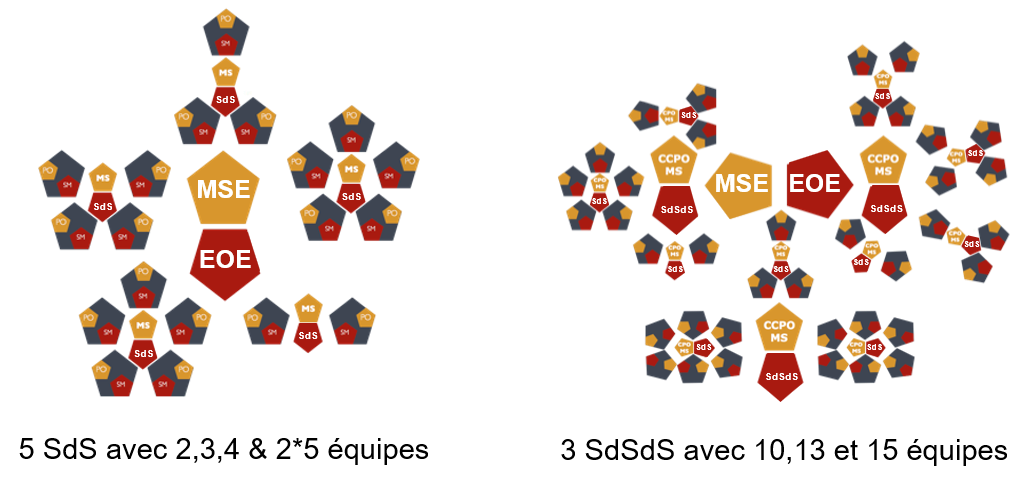
\includegraphics[width=1.0\linewidth]{VariantesSdS-R2.png}
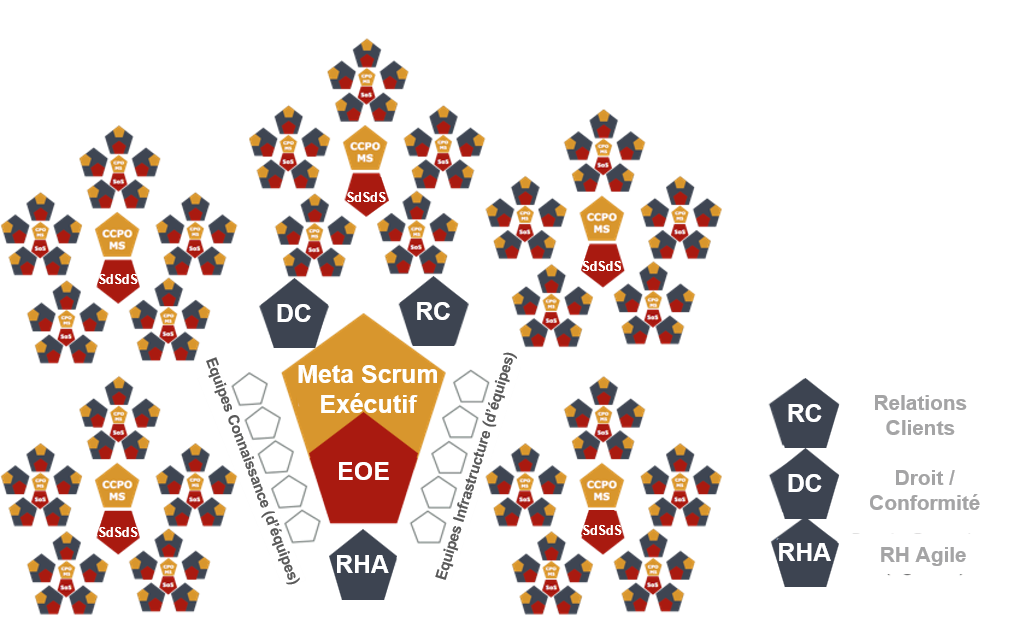
\includegraphics[width=1.0\linewidth]{DiagrammeOrganisationnel.png}

Dans ce schéma organisationnel, les \textbf{équipes Connaissance & Infrastructure}
représentent des équipes virtuelles de spécialistes regroupant du personnel peu assez
nombreux pour créer une équipe à part entière. Elles se coordonnent avec les équipes
Scrum en tant que groupe via des accords de conventions de service où les demandes
passent par un bon de commande pour chaque spécialité qui les convertit en un backlog
ordonné transparent. Il est ici important de remarquer que ces équipes ne sont pas des
silos d'individus physiquement ensemble (c'est pourquoi ils sont représentés comme des
pentagones creux) ; les membres de leur équipe siègent physiquement dans les équipes
Scrum, mais ils constituent leur propre Scrum virtuel à des fins de diffusion du backlog et
de l'amélioration des processus.

Les \textbf{Relations Clients}, le \textbf{Droit / Conformité} et les \textbf{RH Agile} sont incluses car elles sont
parties intégrantes des organisations et existeront en tant qu'équipes indépendantes
Scrum sur lesquelles toutes les autres peuvent compter.

Une note finale sur la représentation des EOE \& MSE : dans ce diagramme, ils sont
présentés comme se chevauchant l’un sur l’autre puisque 2 membres font partis des deux
équipes. Dans les très petites organisations ou implémentations, les EOE \& MSE peuvent
avoir les mêmes membres d'équipe.

\section{Note de fin}
Scrum@Scale est conçu pour augmenter la productivité, pour que l'ensemble de
l'organisation fasse deux fois plus de travail en deux fois moins de temps, avec une qualité
supérieure et un environnement de travail nettement amélioré. Les grandes organisations
qui appliquent correctement le cadre peuvent réduire le coût de leurs produits et services
tout en améliorant la qualité et l'innovation.

Scrum@Scale est conçu pour saturer une organisation avec Scrum. Toutes les équipes, y
compris les équipes Leadership, Ressources humaines, Juridique, Conseil et Formation,
et les équipes produits et services, mettent en oeuvre le même style de Scrum tout en
rationalisant et en améliorant une organisation.

Bien implémenté, Scrum peut gérer toute une organisation.

\section{Remerciements}
Nous remercions IDX pour la création du Scrum de Scrums qui a permis à Scrum
d'atteindre des centaines d'équipes,\footnote{Sutherland, Jeff,
"Inventing and Reinventing SCRUM in five Companies", Sur le site officiel
de l'alliance agile, 2001} PatientKeeper pour la création du MetaScrum,\footnote{Sutherland, Jeff, "Future of scrum: Parallel pipelining
of sprints in complex projects", Proceedings of the Agile Development
Conference,  IEEE Computer Society 90-102,  2005.} qui a
permis le déploiement rapide de produits innovants, et OpenView Venture Partners pour
l'évolution de Scrum vers l'ensemble de l'organisation.\footnote{Sutherland, Jeff and Altman,
Igor, "Take no prisoners: How a venture capital group does scrum", Agile
Conference, 2009. AGILE'09, IEEE 350-355.  2009} Nous apprécions les contributions
d'Intel avec plus de 25 000 personnes pour qui rien n’est extensible, si ce n’est une
architecture libre d’échelle, et SAP avec la plus grande organisation de produits Scrum qui
nous a enseigné que l'implication de la direction dans le MetaScrum est essentielle pour
obtenir 2 000 équipes Scrum travaillant ensemble.

Les coachs et les formateurs agiles implémentant ces concepts chez Amazon, GE, 3M,
Toyota, Spotify et beaucoup d'autres sociétés travaillant avec Jeff Sutherland ont été utiles
pour tester ces concepts dans un large éventail d'entreprises dans différents domaines.

Enfin, Avi Schneier et Alex Sutherland ont été inestimables dans la formulation 
et l'édition de ce document.

\pagebreak

\printbibliography

\pagebreak

\section{Traduction}
\subsection{Lexique}
Il est souvent difficile voire impossible de traduire mot à mot des concepts issus de la
culture anglo-saxonne. Certains mots ont pu être traduits en gardant la sémantique
d’origine, pour d’autres les traducteurs ont dû trouver des mots reliés au sens plus qu’à
cette sémantique. Pour aider le lecteur à retrouver des informations sur internet, nous
avons remis ici les termes d’origine et leur traduction.
Executive Action Team (EAT) : Equipe Opérationnelle Exécutive (EOE)
Executive MetaScrum (EMS) : MetaScrum Exécutif (MSE)
Chief Product Owner CPO : Chef Product Owner (CPO)
Feedback : Retours d’information
Output/Outcomes : Résultats produits / Effets produits
\subsection{Traducteurs}
Les traducteurs agiles : http://www.les-traducteurs-agiles.org/
\begin{itemize}
\item Nicolas Mereaux
\item Laurent Carbonnaux
\end{itemize}

\end{document}
